%% Roman Link's personalized LaTeX Beamer template 
%% contact: rlink@gwdg.de

%% define document class and settings -----------------------------------
\documentclass[usepdftitle=false]{beamer}

%% fonts and input encoding ---------------------------------------------
\usepackage[T1]{fontenc}
\usepackage[utf8x]{inputenc}
\usepackage{lmodern}

%% language support -----------------------------------------------------
\usepackage[english]{babel} % english hyphenation etc.
\usepackage{babelbib}       % multi-language references

%% graphics and colors --------------------------------------------------
\usepackage{graphicx}  
\usepackage{color,pgf}
\usepackage{pdfpages}  % enables the use of pdf graphics

%% mathematical symbols  ------------------------------------------------
\usepackage{amsmath, amsfonts, amssymb, pgf}
\usepackage{eulervm}

%% references with natbib -----------------------------------------------
%\usepackage[round]{natbib}
%\def\newblock{} % hilft gegen absurde fehler mit natbib

%% tweaks of appearance -------------------------------------------------
\usepackage{subscript} % subscripts outside of math expressions
\usepackage{booktabs}  % better-looking tables
\usepackage{ragged2e}  % justified text in Beamer documents with  	
                       % \justifying{}
\usepackage{setspace}  % control line space with spacing environment

%% LaTeX Beamer settings ------------------------------------------------
\mode<presentation>{
	\usecolortheme{seahorse,rose}
	\useinnertheme[shadow]{rounded}
	% \useoutertheme[hideothersubsections,right,width=4em,frame  number]{sidebar}
	% \useoutertheme{infolines}
	% \useoutertheme{split}
	\useoutertheme[subsection=false,footline=authortitle]{miniframes}
	\setbeamercovered{transparent}
}

%% add slide numbers to all slides --------------------------------------
\addtobeamertemplate{navigation symbols}{
  {\usebeamercolor{section in toc}
   \footnotesize
   \insertframenumber/\inserttotalframenumber}
   \hspace{48em}
}{}

%% changes of beamer fonts ----------------------------------------------
\setbeamerfont{section in toc}{size=\normalsize,series=\bfseries}
\setbeamerfont{title}{series=\bfseries}
\setbeamerfont{frametitle}{size=\Large,series=\bfseries}

%% new LaTeX commands ---------------------------------------------------
\newcommand{\sub}[1]{\textsubscript{#1}}
\newcommand{\Sup}[1]{\textsuperscript{#1}}
\newcommand{\COO}{CO\textsubscript{2}}
\newcommand{\masl}{m~a.s.l.}
\newcommand{\gc}{$^{\circ}$C}
\newcommand{\tilt}{$\sim$}
\newcommand{\blue}[1]{{\color{blue!50!black}#1}}
\newcommand{\Blue}[1]{{\color{blue!50!black}\textbf{#1}}}
\newcommand{\eg}{e.\,g.}
\newcommand{\Eg}{E.\,g.}
\newcommand{\rar}{$\rightarrow$}
\newcommand{\lar}{$\leftarrow$}
\newcommand{\Rar}{$\Rightarrow$}
\newcommand{\Lar}{$\Leftarrow$}
\newcommand{\source}[1]{\baselineskip8pt{\tiny \color{gray} #1}}
\newcommand{\tw}{\textwidth}
\newcommand{\ddx}[2]{
	\frac{\mathrm{d}}{\mathrm{d}#2}#1 
	}
\newcommand{\ddxx}[2]{
	\frac{\mathrm{d^2}}{\mathrm{d}#2^2}#1
	}
\newcommand{\code}[1]{
	{\footnotesize 
	 \color{blue}
   \texttt{#1}}
   \normalsize
   \color{black}
  }

%% new environment for slides with changed margins ----------------------
\newenvironment{changemargin}[2]{%
	\begin{list}{}{%
			\setlength{\topsep}{0pt}%
			\setlength{\leftmargin}{#1}%
			\setlength{\rightmargin}{#2}%
			\setlength{\listparindent}{\parindent}%
			\setlength{\itemindent}{\parindent}%
			\setlength{\parsep}{\parskip}%
		}%
		\item[]}
	{\end{list}
}

%% pdf information  -----------------------------------------------------
\hypersetup{
	pdfauthor={Roman M. Link},
	pdftitle={Drought in tropical forests},
}

%% title page settings --------------------------------------------------
\title{Drought in tropical forests}
\subtitle{\normalfont The role of tree height and wood density for hydraulic efficiency, productivity and vulnerability to cavitation of trees along a lowland precipitation gradient}
\author[R. Link]{Roman Link}
\date{January 25, 2018}
\institute[University of Göttingen]{
Department of Plant Ecology and Ecosystem Research\\ Georg August University of Göttingen}
%\titlegraphic{ \vspace*{2em}
%\includegraphics[width=0.7\textwidth]{logouni.png}}
% logo - shown on all pages
\logo{\includegraphics[width=20em]{logo_uni_goe_transparent.png}}

%% start of document ----------------------------------------------------
\begin{document}

%% insert title page ----------------------------------------------------
\begin{frame}
\titlepage
\end{frame}

%% begin of regular slides ----------------------------------------------
\begin{frame}
	\frametitle{Structure of my PhD project}
	\begin{itemize}
		\item<+-| alert@+> Introduction
		\item<+-| alert@+>  \Blue{Chapter 1:} Predicting radial sap flow profiles from Costa Rican tropical dry forest species
		\item<+-| alert@+>  \Blue{Chapter 2:} Estimating plant vulnerability to embolism in Costa Rican humid tropical forest species
		\item<+-| alert@+>  \Blue{Chapter 3:} Relationship between productivity, structural and functional, wood anatomical and hydraulic traits of tropical forest species from Costa Rica
		\item<visible@+-> \Blue{Bonus Chapter:} 
		\alert<5>{Maximum-likelihood estimation of xylem vessel lengths}\visible<6>{: \alert<6>{\textbf{Not in the focus of this presentation!}}
		}
    \end{itemize}	
\end{frame}

\section{Introduction}
\begin{frame}
	\frametitle{Introduction}
	\begin{itemize}
		\item Basics about plant water relations
		\item Why is it important to know about drought effects in the tropics?
	\end{itemize}
\end{frame}

\begin{frame}
	\frametitle{Main research questions}
	\begin{itemize}
		\item This one's gonna be tough
	\end{itemize}
\end{frame}

\begin{frame}
	\frametitle{Design of the study}
	\begin{minipage}{0.5\tw}
		\begin{itemize}[<+-| alert@+>]
			\item 5 research sites along a rainfall gradient on the Pacific shoreline of Costa Rica 			
			\item Gradient from tropical dry forest to humid tropical lowland forest
			\item Based on existing research sites of the \Blue{Instituto Tecnológico de Costa Rica}
		\end{itemize}		
	\end{minipage}
	\begin{minipage}{0.48\tw}
		\includegraphics[width = \tw]{figures/map_01_all_sites.png}  	
	\end{minipage}
\end{frame}

\begin{frame}
	\frametitle{Design of the study}
	\begin{minipage}{0.5\tw}
		\textbf{ At each of the 5 research sites:}
		\begin{itemize}[<+-| alert@+>]
			\item 8 species representing a gradient in tree height and wood density
			\item 5 replicates per species
			\item[\Rar] 40 trees per site, 200 trees in total
		\end{itemize}	
	\end{minipage}
	\begin{minipage}{0.48\tw}
		\includegraphics[width = \tw]{figures/map_01_all_sites.png}  	
	\end{minipage}
\end{frame}


\begin{frame}
	\frametitle{Design of the study}
	\begin{itemize}
		\item \Blue{Variables measured at all sites}
		\begin{itemize}
			\item \alert<1>{Tree level}
			\begin{itemize}
				\item Diameter at breast height
				\item Tree height
				\item Tree growth (basal area/aboveground biomass increment)
				\item Wood density
				\item Sapwood non-structural carbohydrate (NSC) content
			\end{itemize}
			 \item  \alert<1>{Site level}
			  \begin{itemize}
			  	\item Temperature
			  	\item Relative humidity 
			  	\item Precipitation
			  \end{itemize}
		\end{itemize}		
		\item<2> \Blue{Variables measured at a subset of sites}
		\begin{itemize}
			\item  \alert<2>{Sap flow} (only at one site)
			\item  \alert<2>{Branch vulnerability to embolism} (only at two sites)
		\end{itemize}
	\end{itemize}
\end{frame}

\begin{frame}
	\frametitle{Problems with the design}
	\begin{itemize}
		\item<+-> \alert<1>{Opportunistic use of pre-existing plots}
		\begin{itemize}
			\item<+-| alert@+> Different plot sizes and numbers at each site
			\item<+-| alert@+> Differences in historic land use (pristine primary forest vs. disturbed primary forest vs. secondary forest)
			\item<+-| alert@+> Cooperation with forestry department (foresters do forester things...)
		\end{itemize}	
		\item<visible@+-| alert@+>[\rar] Plot-based comparisons are difficult
		\item<visible@+-| alert@+>[\Rar] Not that important for our (eco-physiological) research questions, but limits usability of plot network for other research areas
	\end{itemize}
\end{frame}


\section{Radial sap flow profiles}
\begin{frame}
	\frametitle{First chapter: radial sap flow profiles}
	\begin{minipage}{0.5\tw}
	 \textbf{Sap flow measurements:}
	 \begin{itemize}
	 	\item<+-| alert@+> Practical limitations \rar\ only in dry forest (Horizontes)
	 	\item<+-| alert@+> 4 measurement campaigns of $\pm$ 1 week during rainy season of 2015
	 	\item<+-| alert@+> 40 trees of 8 species	
	 	\item<+-| alert@+> Measured with the Heat Field Deformation (HFD) method			
	 \end{itemize}			
	\end{minipage}
	\begin{minipage}{0.48\tw}
		\only<1>{\includegraphics[width = \tw]{figures/map_02_horizontes.png}} 	
		\only<2-3>{\includegraphics[width = \tw]{figures/Guanacaste2015.jpg}\\
			
			\source{Image source: Instituto Meteorológico Nacional de Costa Rica}} 			
		\only<4>{\centering 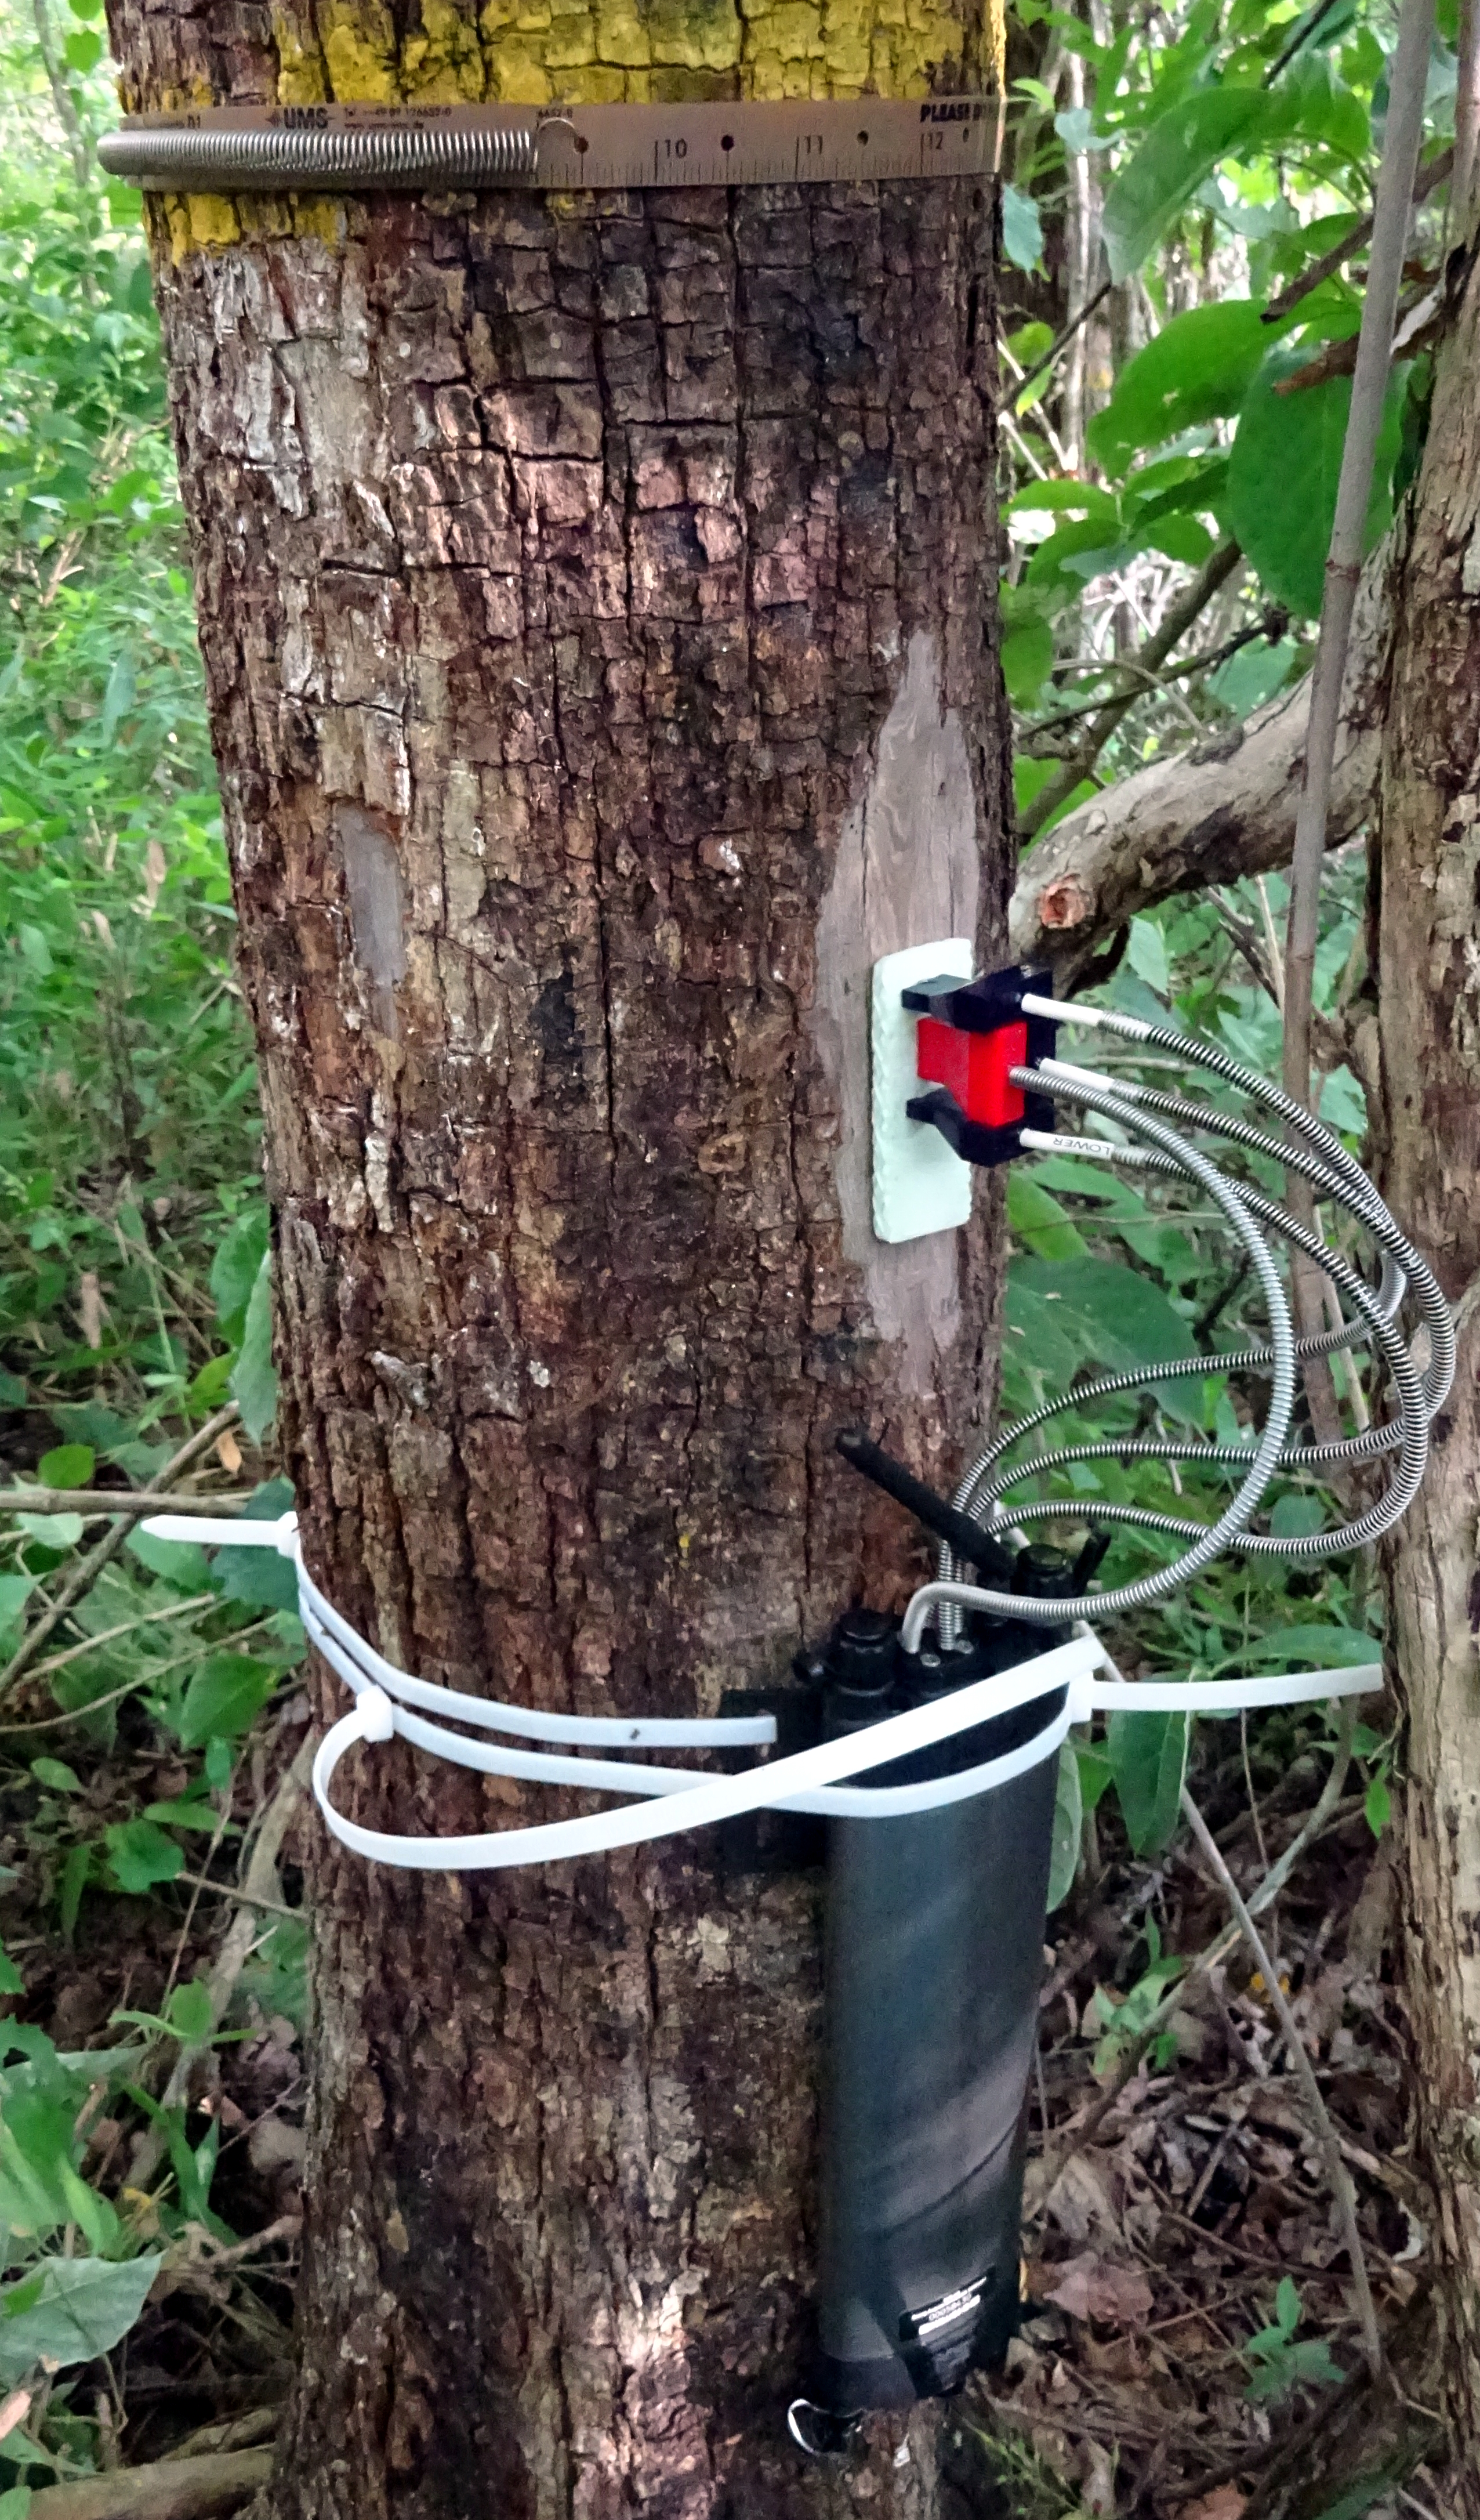
\includegraphics[width = 0.7\tw]{figures/HFD_01_sensor.JPG}}
	\end{minipage}
\end{frame}

\begin{frame}	
	\includegraphics[height = \textheight]{figures/horizontes_WD_height1.png}
\end{frame}


\begin{frame}
	\frametitle{Heat field deformation sensors}
	\begin{minipage}{0.5\tw}
		\textbf{Working principle:}
		\begin{itemize}
			\item<+-| alert@+> 1 heater and 3 temperature sensors inserted into wood
			\item<+-| alert@+> Heater heats constantly with known caloric input
			\item<+-| alert@+> Sap movement \rar\ faster heat transport in flow direction
			\item<+-| alert@+> Temperature differences between sensors are used for estimation of sap flux density at different depths
		\end{itemize}						
	\end{minipage}
	\begin{minipage}{0.48\tw}
			\only<1-2>{\includegraphics[width = \tw]{figures/nadezhdina_01.png}}
			\only<3-4>{\quad\quad \includegraphics[width = 0.6\tw]{figures/nadezhdina_02.png}}\\
				
				\source{Image source: Nadezhdina et al., 2012}
	\end{minipage}
\end{frame}

\begin{frame}[t]
	\frametitle{Heat field deformation sensors}
	\begin{itemize}
		\item<only@1| alert@1> Original idea: Comparison of sap flow and plant water use between species with different trait combinations
		\item<only@2-> Problem: newer research indicates that
		\begin{itemize}
			\item[a)]<2-| alert@2> The mechanistic explanation of the HFD method (Nadezhdina et al., 2012) is flawed (Vandegehuchte \& Steppe, 2012)\\ \rar\ species-specific calibration likely necessary in most cases
			\item[b)]<3-| alert@3> HFD calibration parameters are not consistent within species (Fuchs et al., 2017)
		\end{itemize}	
		\item<only@4-| alert@4>\textit{ Relative values} are probably reliable, \textit{absolute values} have to be handled with care
		\item<only@5| alert@5>[\Rar] \textbf{Decision for analysis: better to put focus on radial gradients of sap flux}
	\end{itemize}
	\only<2>{\includegraphics[width = \tw]{figures/vandegehuchte_01.png}}
  \only<3>{\includegraphics[width = \tw]{figures/HFDSeb_01_paper.png}}	
\end{frame}

\begin{frame}
	\frametitle{Research questions \& hypotheses}
	\begin{minipage}{0.38\tw}
		\includegraphics[width = \tw]{figures/HFD_05_profile_simarouba.png}
	\end{minipage}
	\begin{minipage}{0.6\tw}
			\begin{itemize}
			\item Radial sap flow gradients
			\begin{itemize}[<+-| alert@+>]
				\item very important for studies of plant water use
				\item few methods take them into account
				\item sensors are expensive and error-prone
			  \item species specific measurement: problematic in the tropics		
			\end{itemize}
			\item<+-| alert@+>[\Rar] \Blue{Question:} Is it possible to predict the shape of radial sap flow profiles based on tree traits?
			\item<visible@+| alert@+>[\Rar] \Blue{Hypothesis:} The shape of radial sap flow profiles depends on \textbf{wood density} and \textbf{tree height}
		\end{itemize}						
	\end{minipage}
\end{frame}

\begin{frame}
	\frametitle{Data analysis}
	\begin{minipage}{0.38\tw}
		\includegraphics[width = \tw]{figures/HFD_05_profile_simarouba.png}
	\end{minipage}
	\begin{minipage}{0.6\tw}				
		\begin{itemize}[<+-| alert@+>]
			\item Nonlinear relationship
			\item Parameters that control the shape of the nonlinear relationship depend on other variables
			\item Hierarchical data structure (repeated observations in replicate trees from different species)		
			\item<visible@4| alert@4>[\Rar] \textbf{How to analyze?}
		\end{itemize}
	\end{minipage}
\end{frame}

\begin{frame}[t]
	\frametitle{Data analysis}
	\begin{itemize}
		\item Analysis based on \Blue{Bayesian nonlinear hierarchical models}
		\begin{itemize}			
			\item<2-> \alert<2>{\textbf{First stage of the model:}} Nonlinear relationship between sensor depth and predicted flux density modeled by density function of the Weibull distribution
			\item<3->  \alert<3>{\textbf{Second stage of the model:}} Parameters of the Weibull distribution modeled as a function of wood density, tree height and their interaction, accounting for species and stem specific random variation
			\item<only@4->  \alert<4>{Model fitting with the \textbf{Stan modeling language}}
		\end{itemize}
		\item<only@5| alert@5> Models still need tuning \rar\ shown results are from preliminary model based on R package \texttt{nlme}
	\end{itemize}
	  \only<2-3>{\includegraphics[width = 0.8\tw]{figures/weibulldens.png}}
\end{frame}

\begin{frame}
	\frametitle{Model equations of the preliminary model}
  \includegraphics[height=0.9\textheight]{figures/HFD_06_model.png}
\end{frame}

\begin{frame}
	\includegraphics[height=\textheight]{figures/HFD_02_profiles.png}
\end{frame}

\begin{frame}
	\frametitle{Preliminary results I - predicted profiles}	
	\begin{minipage}{0.6\tw}
		\begin{itemize}[<+-| alert@+>]
			\item Model explains a large part of the observed variance in the dataset (conditional pseudo-R\Sup{2} = 0.918)
			\item Most of this variance is explained by random differences between species and stems (marginal pseudo-R\Sup{2} = 0.329)
		\end{itemize}						
	\end{minipage}
	\begin{minipage}{0.38\tw}
		\includegraphics[width = \tw]{figures/HFD_05_profile_simarouba.png}
	\end{minipage}	
\end{frame}

\begin{frame}[t]
	\frametitle{Preliminary results II - parameter models}
		\only<1>{\includegraphics[width=\tw]{figures/HFD_03a_k_responses.png}}
		\only<2>{\includegraphics[width=\tw]{figures/weibulldens_K.png}}
		\begin{itemize}
		\item \Blue{Weibull shape parameter K} 
			\begin{itemize}
				\item	No significant height- and wood density effects
			\end{itemize}
	\end{itemize}
\end{frame}

\begin{frame}[t]
	\frametitle{Preliminary results II - parameter models}
  \only<1>{\includegraphics[width=\tw]{figures/HFD_03b_lambda_responses.png}}
	\only<2>{\includegraphics[width=\tw]{figures/weibulldens_lambda.png}}
	\begin{itemize}
		\item \Blue{Weibull scale parameter $\lambda$}
		\begin{itemize}
			\item Decreases significantly with tree height and wood density, but significantly less so in trees that are both large AND have hard wood
		\end{itemize}	
	\end{itemize}
\end{frame}

\begin{frame}
	\frametitle{Radial sap flow profiles - Conclusions}
	\begin{itemize}[<+-| alert@+>]
		\item Shape of the profile significantly depends on height and wood density
		\item Model describes observed radial profiles very well
		\item Explained variance is much lower when predicting onto new trees because of the high stem-specific variability
		\item Inclusion of other predictors might improve predictions (and consequently increase the value of the model for studies of plant water use)
	\end{itemize}
\end{frame}


\section{Vulnerability curves}
\begin{frame}
	\frametitle{Second chapter: vulnerability curves}
	\begin{changemargin}{-1em}{-1em}	
		\centering{
			\includegraphics[width=0.65\tw]{figures/schuldt_2015_VC.png}}
		\begin{itemize}
			\item<only@1> Relationship between \alert{water potential} and \alert{percentage loss of conductivity} (PLC)
			\item<only@1>[\rar] shows the loss of conductive function under increasingly dry conditions
			\item<only@2> \alert{Parameters of vulnerability curves:} important predictors of drought response
			\begin{itemize}
				\item  \Blue{P\sub{50}:} At what pressure 
				does a plant lose 50\% of its conductivity?  
				\item \Blue{Slope:} How fast does this loss occur?
			\end{itemize}
		\end{itemize}  
		\only<2>{\vspace{0.65em}}
		\source{Image source: Schuldt et al., 2015}
	\end{changemargin}	
\end{frame}

\begin{frame}
	\frametitle{Second chapter: vulnerability curves}
	\begin{minipage}{0.5\tw}
			\begin{itemize}
			\item<1-| alert@1> Vulnerability curves of replicate samples from 30 trees of 10 tropical forest species from the Osa peninsula (56 in total)
			\item<2-| alert@2-4> Collection of upper canopy branches in two campaigns in the rainy seasons  of 2016 and 2017
			\item<5-| alert@5-> Measured with the Cavitron method using a novel 1~m rotor (courtesy of the lab of Sylvain Delzon, Bordeaux) 
		\end{itemize}			
	\end{minipage}
	\begin{minipage}{0.48\tw}
		\centering
		\only<1>{\includegraphics[width = \tw]{figures/map_03_osa.png}}	
		\only<2>{\includegraphics[width = 0.75\tw]{figures/field1.jpg}}	
		\only<3>{\includegraphics[width = 0.75\tw]{figures/field2.jpg}}
		\only<4>{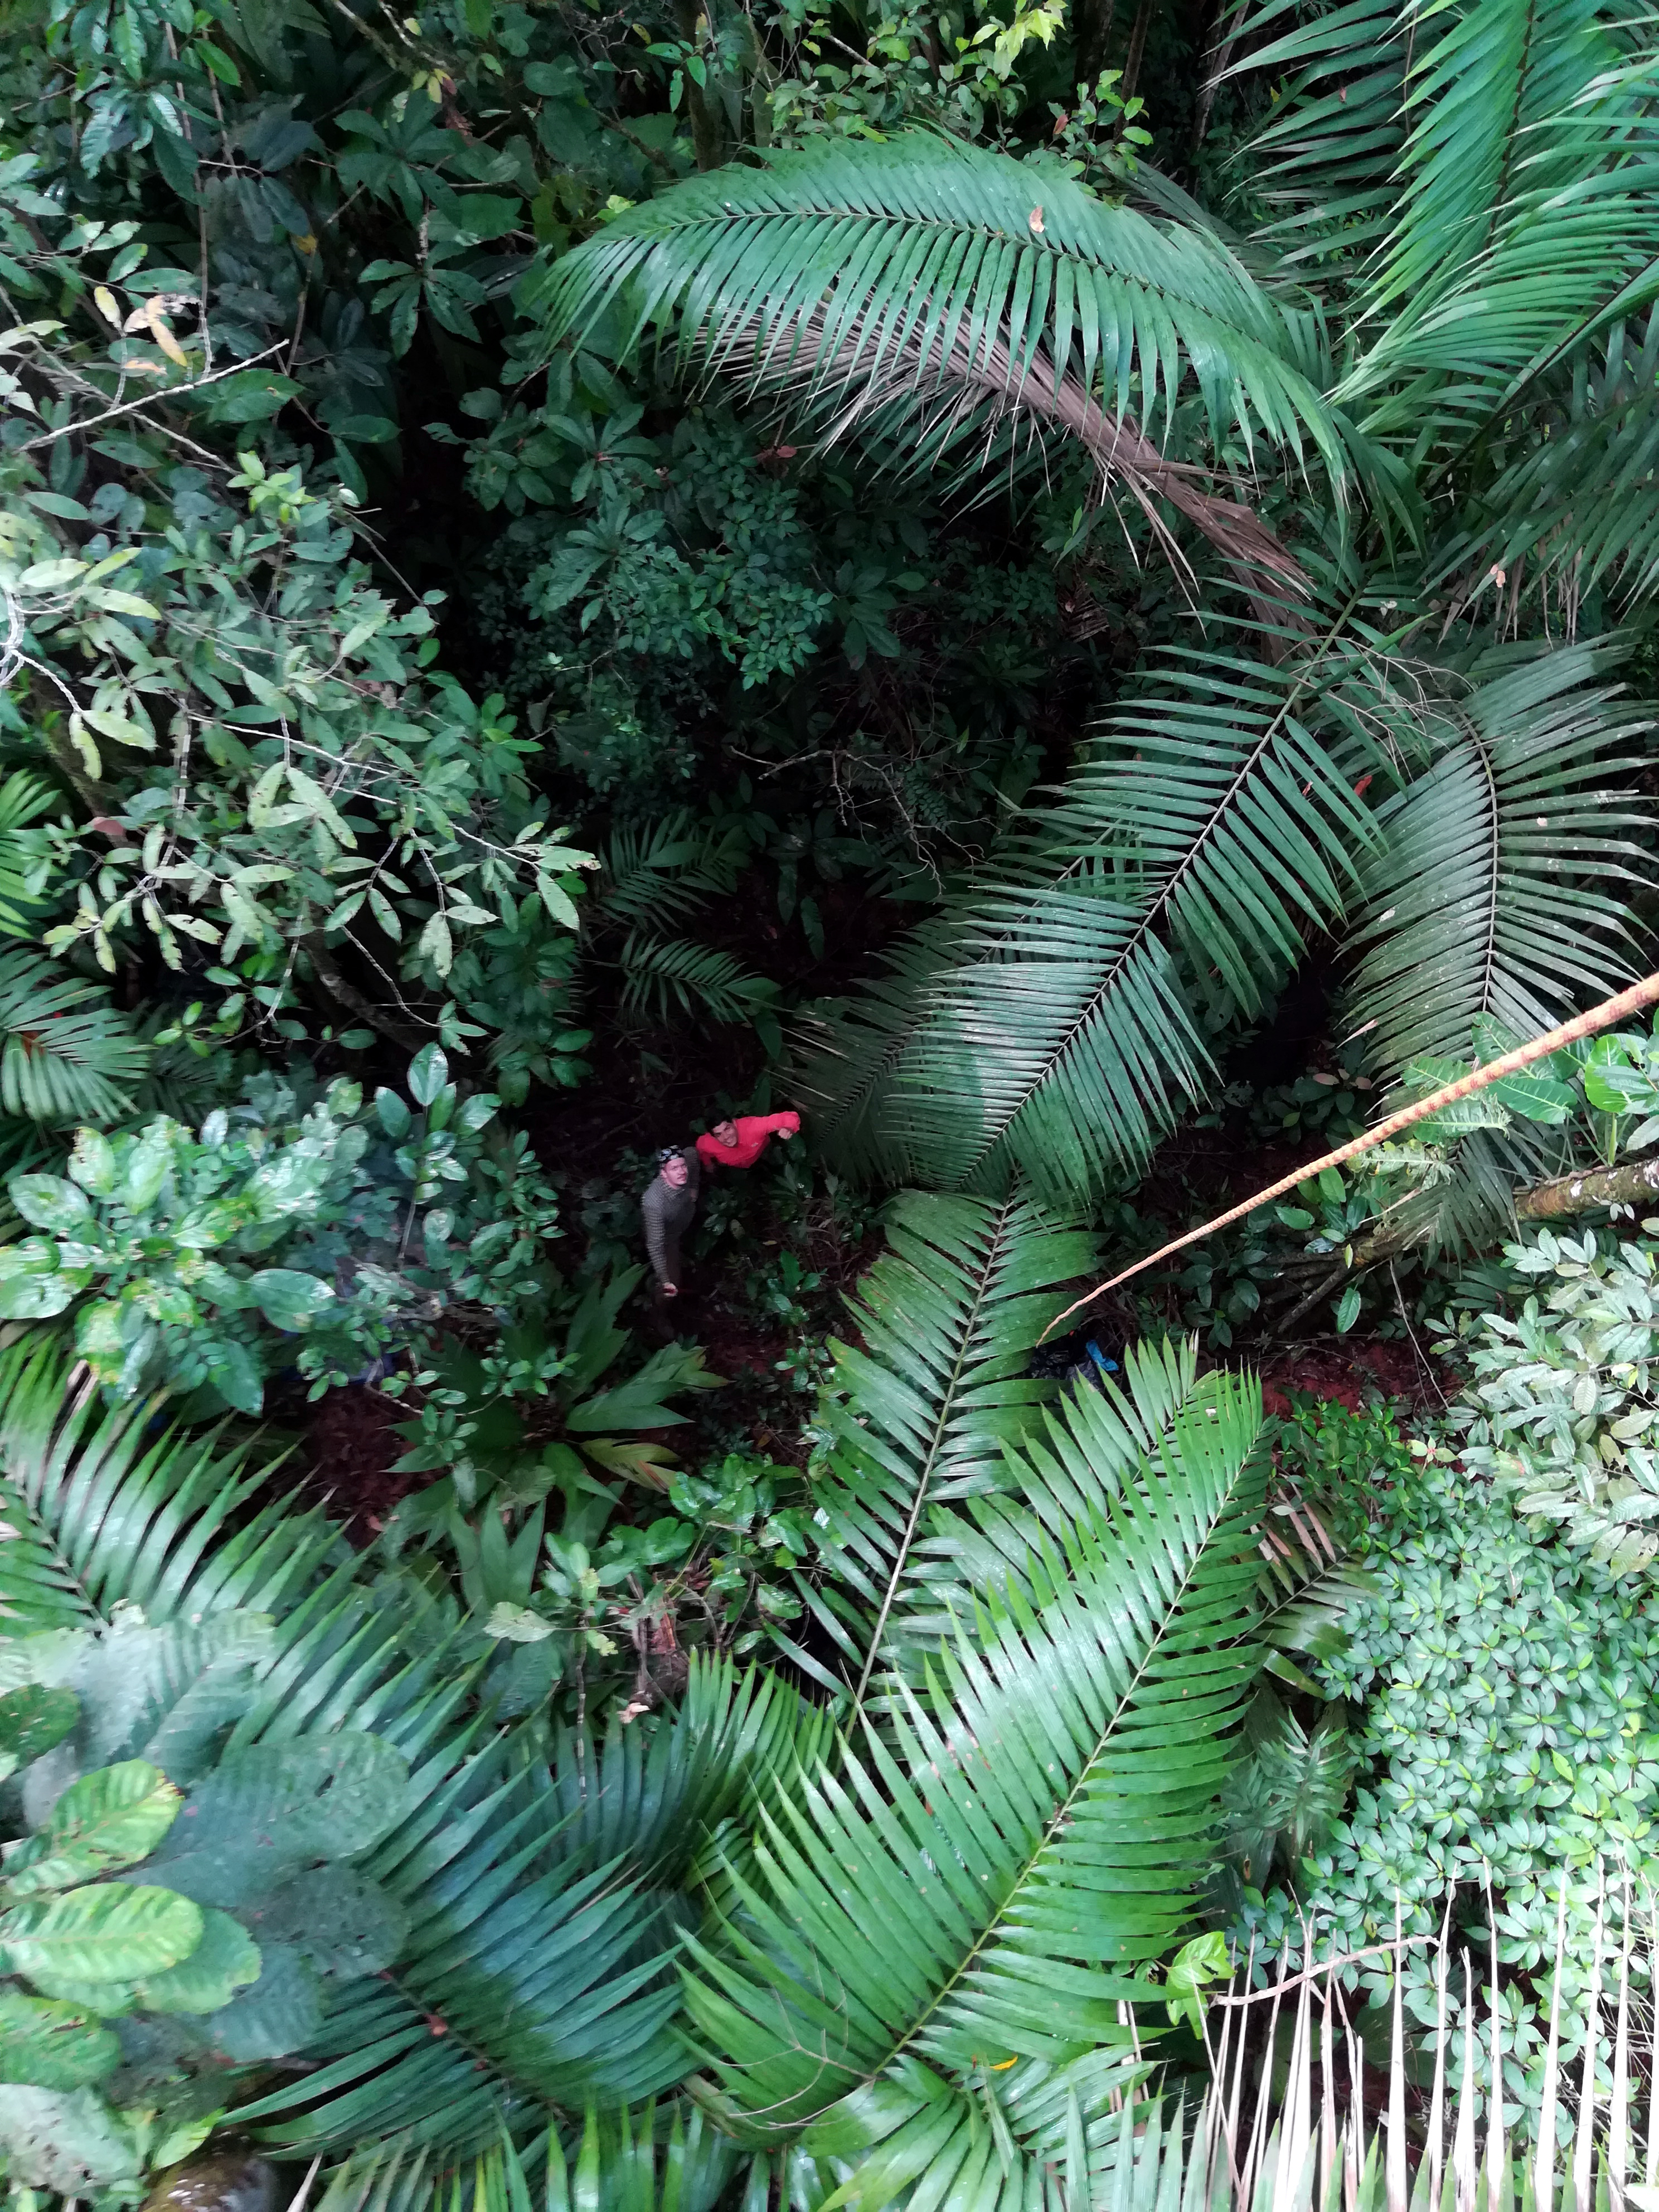
\includegraphics[width = 0.8\tw]{figures/field3.jpg}}
		\only<5>{\includegraphics[width = \tw]{figures/cavi01.jpg}\\			
			\source{Foto: \url{http://sylvain-delzon.com/caviplace/}}}
		\only<6>{\includegraphics[width = 0.9\tw]{figures/cavi02.jpg}\\
			\source{Foto: \url{http://sylvain-delzon.com/caviplace/}}}
		\end{minipage}	
\end{frame}


\begin{frame}
	\frametitle{Research questions \& hypotheses}
	\begin{itemize}
		\item Plant vulnerability to embolism can be predicted by structural, functional and wood anatomical traits
	\end{itemize}
\end{frame}

\begin{frame}
	\frametitle{Data analysis}
	\centering{\includegraphics[width=0.38\tw]{figures/schuldt_2015_VC.png}}
	\begin{itemize}[<+-| alert@+>]
		\item Nonlinear relationship
		\item Parameters that control the shape of the nonlinear relationship (P50 and slope) depend on other variables
		\item Hierarchical data structure (repeated observations on replicate samples from replicate trees belonging to different species)		
		\item<visible@4-| alert@4>[\Rar] \textbf{Nonlinear hierarchical models}\\ (analogous to models for radial sap flow profiles)
		\item<visible@5| alert@5>[\Rar] \textbf{\Large Data analysis in progress}
	\end{itemize}	
	\source{Image source: Schuldt et al., 2015}
\end{frame}

\begin{frame}
	\frametitle{Observed vulnerability curves}
		\includegraphics[height=0.9\textheight]{figures/VC_02_preliminary_plot.jpg}
\end{frame}

\section{The big picture}
\begin{frame}
	\frametitle{The big picture}
	\begin{itemize}
		\item Do structural, functional and wood anatomical traits explain changes in productivity and hydraulic traits? 
		\item How are these changes related to the rainfall gradient?
	\end{itemize}
\end{frame}

\begin{frame}
	\frametitle{Growth data}
	\begin{itemize}
		\item short description
		\item picture
	\end{itemize}
\end{frame}

\begin{frame}
	\frametitle{Wood anatomy}
	\begin{itemize}
		\item short description
		\item picture
	\end{itemize}
\end{frame}

\begin{frame}
	\frametitle{Non-structural carbohydrates}
	\begin{itemize}
		\item short description
		\item picture
		\item data not available so far
	\end{itemize}
\end{frame}

\begin{frame}
	\frametitle{Research questions \& hypotheses}
	\begin{itemize}
		\item Lots and lots of hypotheses
	\end{itemize}
\end{frame}

\begin{frame}
	\frametitle{Data analysis}
	\begin{itemize}
		\item Short explanation of structural equation models		
	\end{itemize}
\end{frame}

\begin{frame}
	\frametitle{Meta-model \& causal diagram}
	\begin{itemize}
		\item figures on one or two slides		
	\end{itemize}
\end{frame}

\begin{frame}
	\frametitle{Example for SEM: Martyna's paper}
	\begin{itemize}
		\item Meta-model, causal diagram \& final path model	
	\end{itemize}
\end{frame}

\begin{frame}
	\frametitle{Summary}
	\begin{itemize}
		\item Sap flow
		\item Vulnerability curves
		\item SEM
	\end{itemize}
\end{frame}


\begin{frame}
	\frametitle{Thanks \& goodbye}
	\begin{itemize}
		\item Names of assistants (pictures?)
	\end{itemize}
\end{frame}

\section{References}
\begin{frame}
	\frametitle{References}
	\begin{itemize}
		\item \textbf{Fuchs S, Leuschner C, Link R, Coners H, Schuldt B, 2017.}
		Calibration and comparison of thermal dissipation, heat ratio and heat field deformation sap flow probes for diffuse-porous trees,
		\textit{Agricultural and Forest Meteorology} \textbf{244–245},151-161. \url{https://doi.org/10.1016/j.agrformet.2017.04.003.}.
	\end{itemize}
\end{frame}
\end{document}
